\section{Literature Review}
\label{sec:related_work}

\subsection{MoCo: Momentum Contrast for Unsupervised Visual Representation Learning}

Momentum Contrast (MoCo) \cite{he2020momentum} is a self-supervised learning framework built on the idea of contrastive learning. MoCo maintains a dynamic dictionary of negative samples using a momentum-based encoder. This dictionary is implemented as a queue, where old representations are progressively replaced by new ones. The novelty that MoCo introduces in its momentum encoder, which helps maintain consistency in feature representations over time and reduces memory constraints by allowing the model to use a relatively smaller batch size while still accessing a large pool of negative samples.

\begin{figure}[t]\centering
\vspace{1.em}
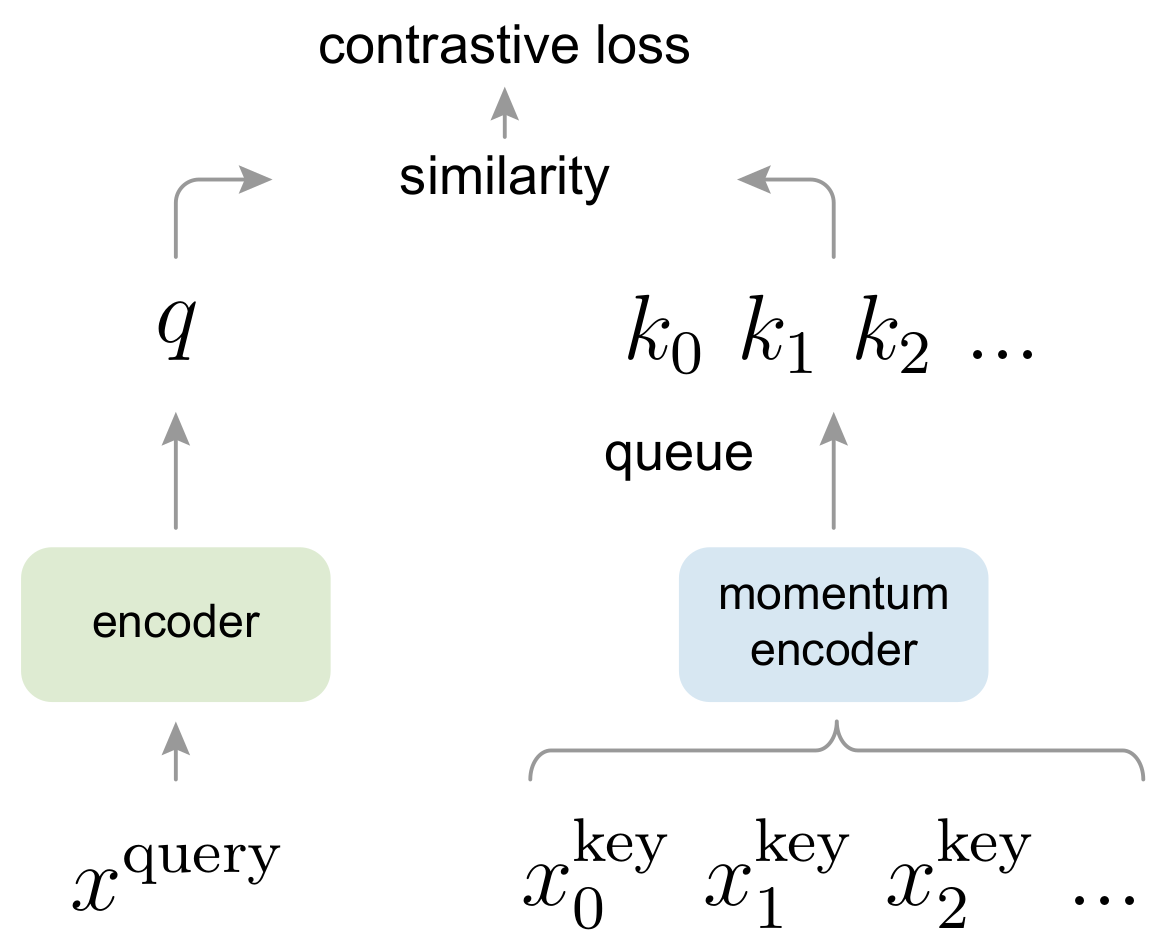
\includegraphics[width=.65\linewidth]{images/MoCo_Architecture.png}
\caption{Momentum Contrast (MoCo) trains a visual representation encoder by matching an encoded query $q$ to a dictionary of encoded keys using a contrastive loss. The dictionary keys $\{k_0, k_1, k_2, ...\}$ are defined on-the-fly by a set of data samples.
The dictionary is built as a queue, with the current mini-batch enqueued and the oldest mini-batch dequeued, decoupling it from the mini-batch size.
The keys are encoded by a slowly progressing encoder, driven by a momentum update with the query encoder.
This method enables a large and consistent dictionary for learning visual representations.
\label{fig:teaser}}
\vspace{-1em}
\end{figure}

The MoCo architecture consists of two encoders: a query encoder and a key encoder. The query encoder is updated via backpropagation, while the key encoder is updated using an exponential moving average (momentum update) to ensure stability as follows:
\begin{equation}
\theta_\textrm{k} \leftarrow m \theta_\textrm{k} + (1 - m) \theta_\textrm{q}.
\label{eq:moco}
\end{equation}
Given an image, two different augmentations are applied, producing a query image and a key image. The query image is encoded using the query encoder, and the key image is encoded using the momentum encoder. The contrastive loss, typically InfoNCE defined as follows:
\begin{equation}
\mathcal{L}_q = -\log \frac{\exp(q{\cdot}k_+ / \tau)}{\sum_{i=0}^{K}\exp(q{\cdot}k_i  / \tau)}
\label{eq:infonce}
\end{equation}
This loss is then applied to maximize similarity between the query and key embeddings while minimizing similarity with a queue of negative samples. This framework has been widely adopted in self-supervised learning due to its efficiency in handling large-scale datasets with limited computational resources.

\subsection{Learning features by Swapping Assignments between multiple Views (SwAV) of an Image}

SwAV (Swapping Assignments Between Views) \cite{caron2020unsupervised} is a self-supervised learning method that introduces a clustering-based approach to learning visual representations without explicit contrastive loss. SwAV directly learns cluster assignments for different augmentations of the same image. This is achieved by using a swapped prediction mechanism, where the model predicts the cluster assignment of one view using the features of another as seen in the loss function:
\begin{eqnarray}
L(\mathbf{z}_t, \mathbf{z}_s) & = &\ell(\mathbf{z}_t, \mathbf{q}_s) + \ell(\mathbf{z}_s, \mathbf{q}_t),
\label{eq:twoviews}
\end{eqnarray}

The terms in the loss function representing the swapped prediction terms are defined as the cross-entropy loss between the code and the probability obtained by taking a softmax of the dot products of ${z_i}$ and all prototypes in C (set of learned prototypes). Some improvements that the SwAV paper proposes firstly is computing the codes in an online fashion and secondly is the choice of another image augmentation, namely Multi-crop. In the multi-crop strategy we use two standard resolution crops and sample additional low resolution crops that cover only small parts of the image because comparing random crops of an image plays a central role by capturing information in terms of relations between parts of a scene or an object.

\begin{figure}[t]
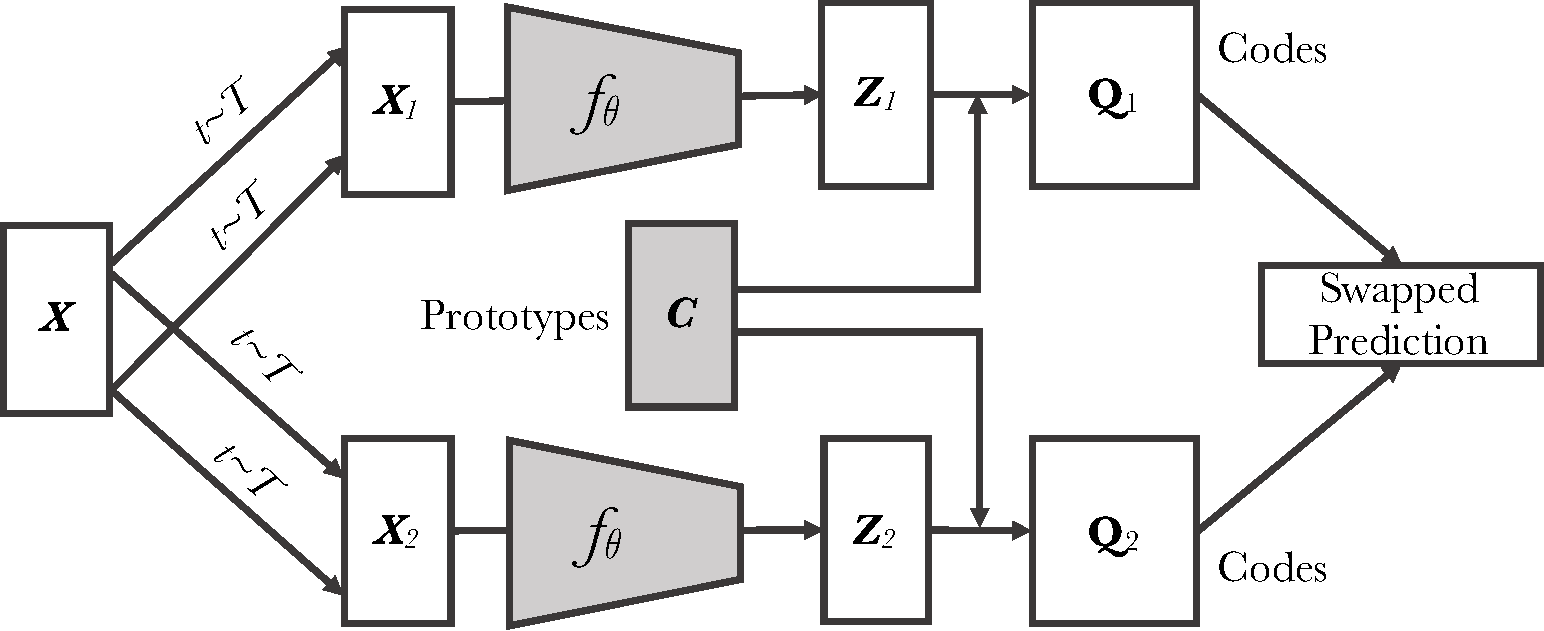
\includegraphics[height=.4\linewidth]{images/oto_simple.pdf}
\caption{
We first obtain ``codes'' by assigning features to prototype vectors.
We then solve a ``swapped'' prediction problem wherein the codes obtained from one data augmented view are predicted using the other view.
Prototype vectors are learned along with the ConvNet parameters by backpropragation. 
}
\end{figure}

\subsection{Prototypical Part Network (ProtoPNet)}

Prototype Part Networks (ProtoPNet) \cite{chen2019looks} introduce a novel interpretable deep learning framework by integrating prototype-based reasoning into convolutional neural networks (CNN). ProtoPNet learns a set of class-specific prototype representations, which correspond to meaningful image patches. During inference, an input image is compared with these prototypes, and classification is performed based on similarity scores. This approach provides inherent interpretability by allowing visualization of the prototypical features that influence model predictions. The network is trained using a combination of standard cross-entropy loss and a specialized prototype loss, ensuring that learned prototypes remain discriminative and aligned with human-interpretable visual concepts. 

\begin{figure*}[t]\centering
\vspace{1.em}
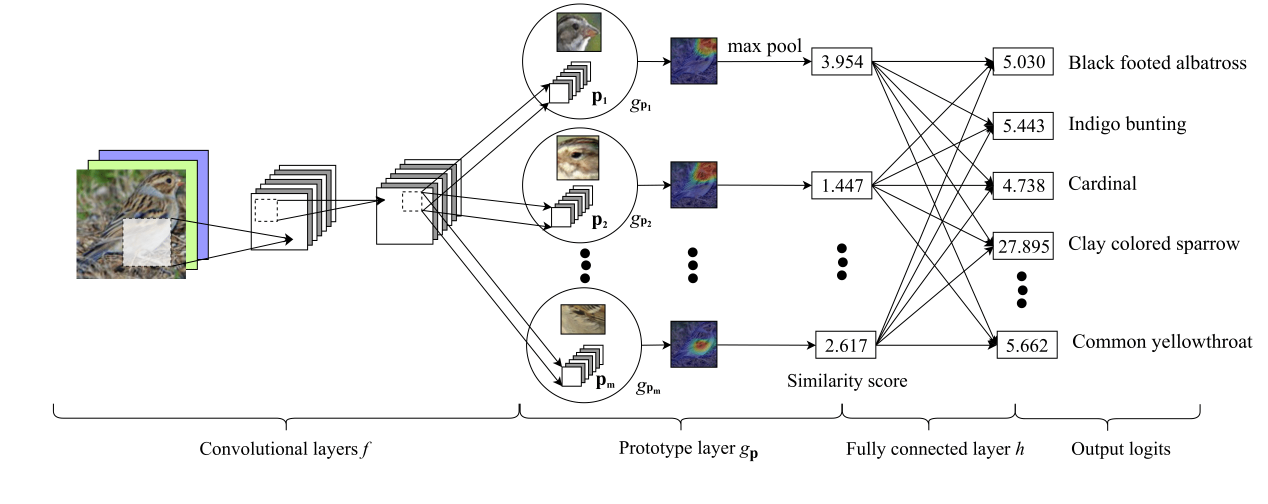
\includegraphics[width=.75\linewidth]{images/ProtoPNet_Architecture.png}
\caption{ProtoPNet Architecture
\label{fig:teaser}}
\vspace{-1em}
\end{figure*}

The issue in using the ProtoPNet net is that we assume that our data to be unlabeled and hence will be unable to use the class specific prototype representations the model learns. Though the general idea of using prototype learning in self-supervised learning does prove to be useful and can be seen in other papers like Protocon \cite{nassar2023protocon}.